%–––––––––––––––––––––––––––––––––––––––––––––––
% content/01_introduction.tex
%–––––––––––––––––––––––––––––––––––––––––––––––

\section{Introduction}


\begin{frame}[t, fragile]
  \frametitle{Introduction to Lung CT}

  \begin{itemize}
    \item<1-> \textbf{Lung CT Reconstruction}: The reconstruction of lung CT images can be formulated as the following optimization problem:
          \begin{equation*}
            \min_{\textcolor{green}{\boldx}} \frac{1}{2}\left\| \boldcalR \textcolor{green}{\boldx} - \boldb \right\|_{W}^2 + \boldR(\textcolor{green}{\boldx})
          \end{equation*}
    \item<2-> \textbf{Limitations of Static CT}:
          \begin{itemize}
            \item Assumes the patient remains stationary during the scan.
            \item Respiratory motion can introduce artifacts and blurring.
          \end{itemize}
    \item<3-> \textbf{Introduction to 4DCT}:
          \begin{itemize}
            \item Captures 3D images across respiratory phases, enabling dynamic lung motion visualization.
            \item Essential for applications like radiotherapy planning \cite{kwong2015f}.
          \end{itemize}
  \end{itemize}
\end{frame}

\begin{frame}[t, fragile]

  \frametitle{Introduction to Dynamic Lung CT}

  \begin{itemize}
    \item<1-> \textbf{4DCT Acquisition Modes}:
          \begin{itemize}
            \item Helical mode: The scanner rotates continuously as the patient table moves through the gantry.
            \item Cine mode: The scanner acquires multiple images at the same table position over a period.
            \item Uses a surrogate signal (e.g., respiratory belt or external marker) to track breathing motion.
          \end{itemize}
    \item<2-> \textbf{Example of Helical 4DCT Acquisition}:

  \end{itemize}

  \only<3>{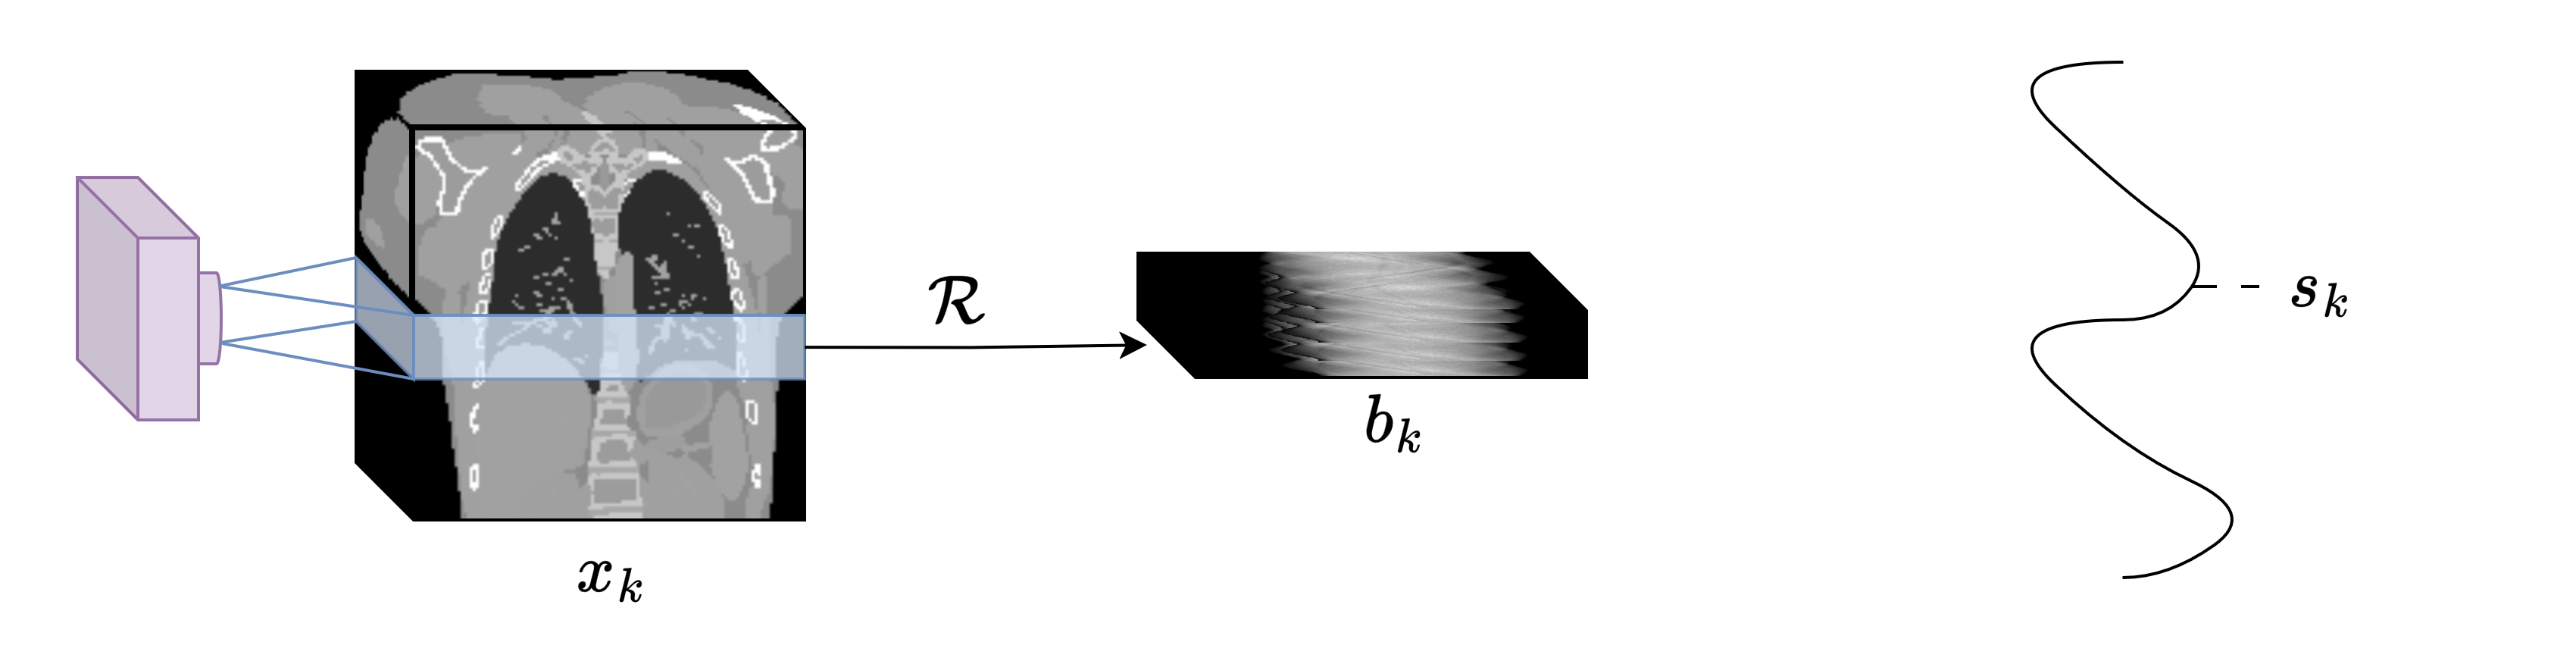
\includegraphics[width=1\linewidth]{figures/intro/acquisition/acqu1.png}}
  \only<4>{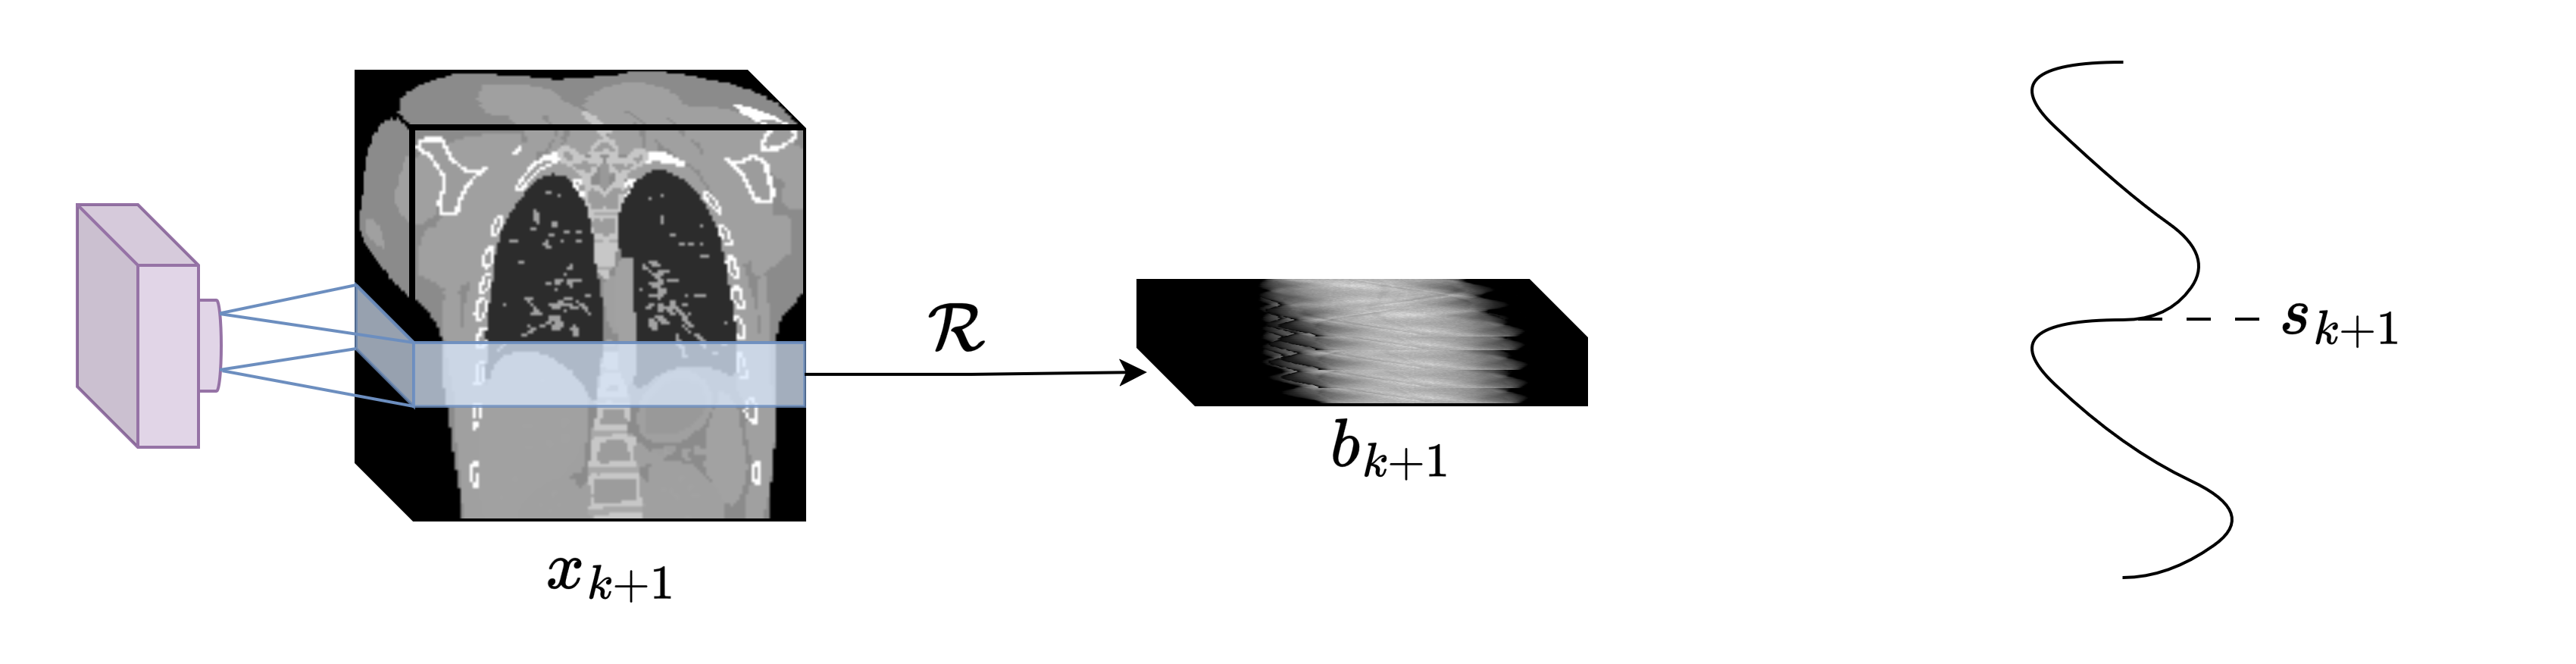
\includegraphics[width=1\linewidth]{figures/intro/acquisition/acqu2.png}}
  \only<5>{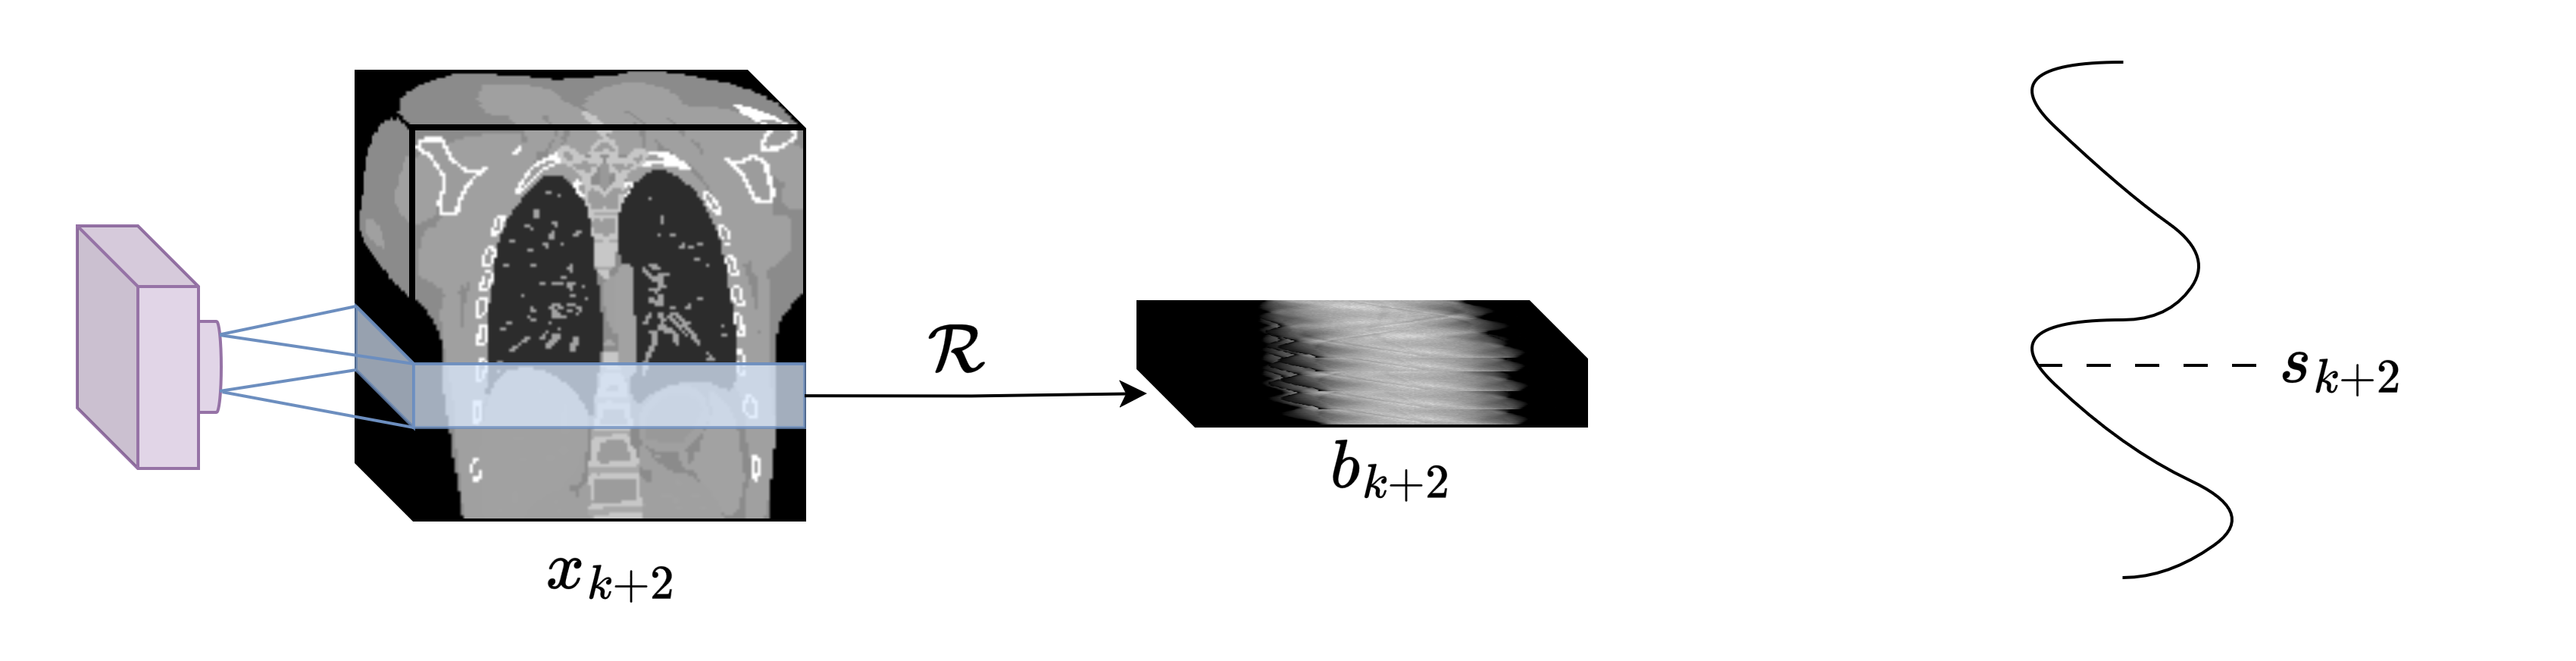
\includegraphics[width=1\linewidth]{figures/intro/acquisition/acqu3.png}}
  \only<6>{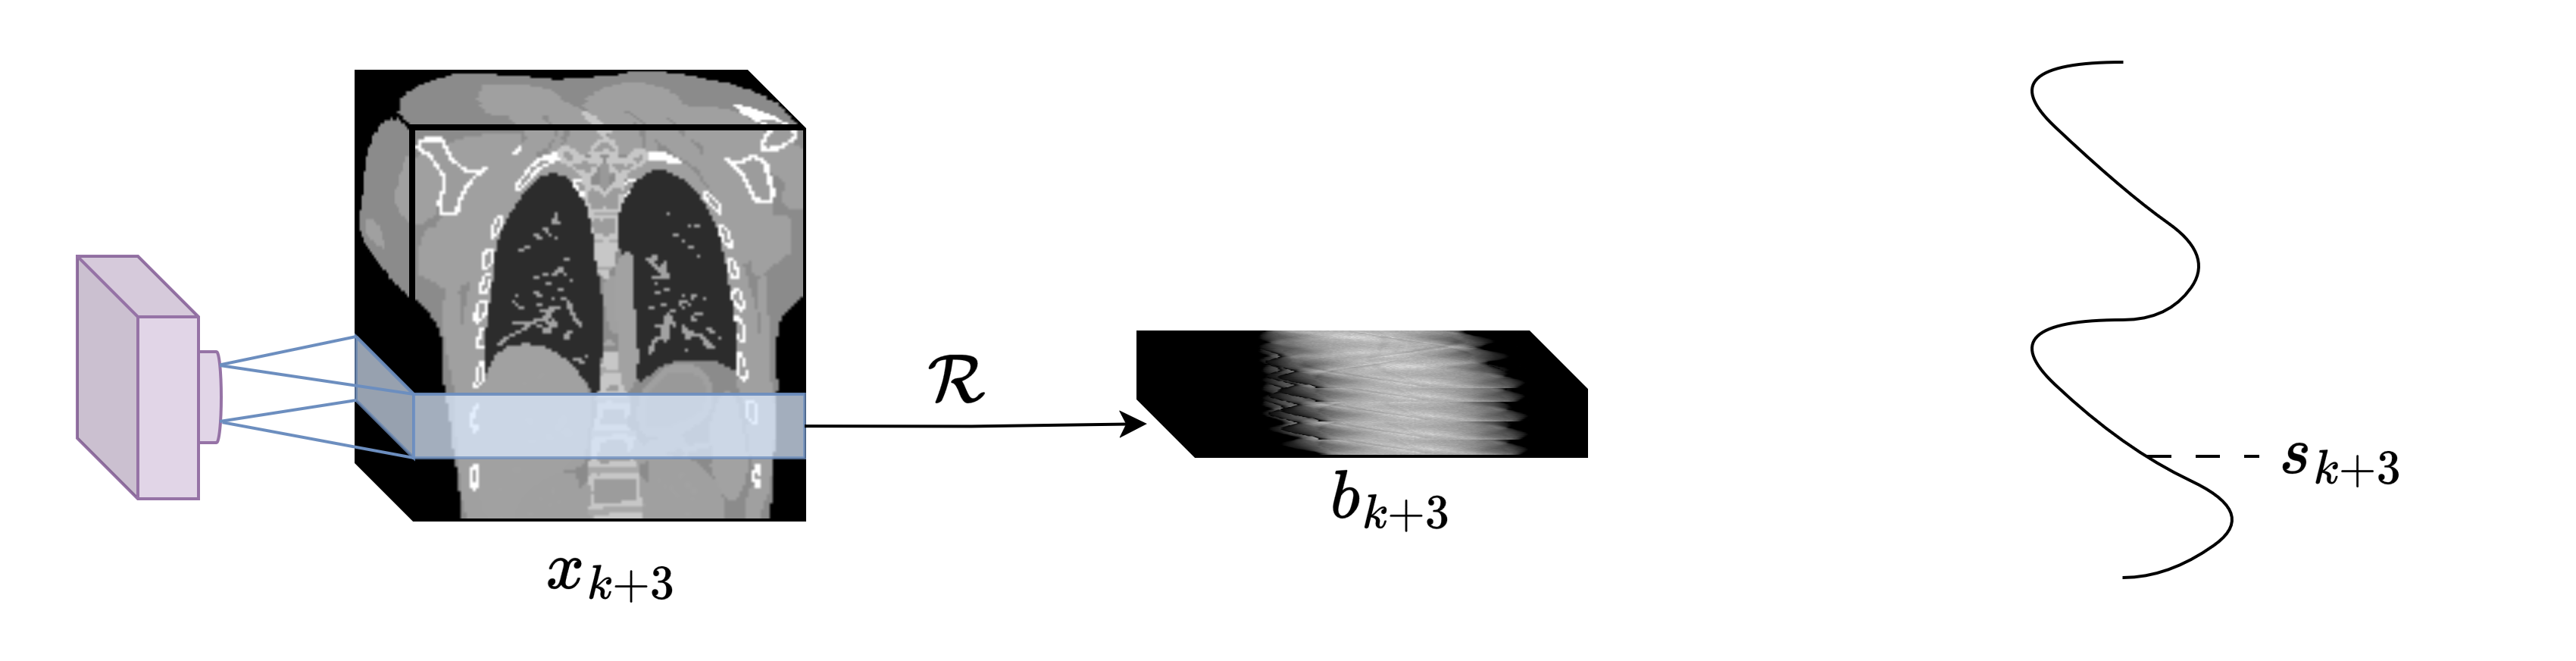
\includegraphics[width=1\linewidth]{figures/intro/acquisition/acqu4.png}}

\end{frame}



\begin{frame}[t, fragile]
  \frametitle{Challenges in 4DCT}

  % Show first two images only on specific overlays
  \only<1>{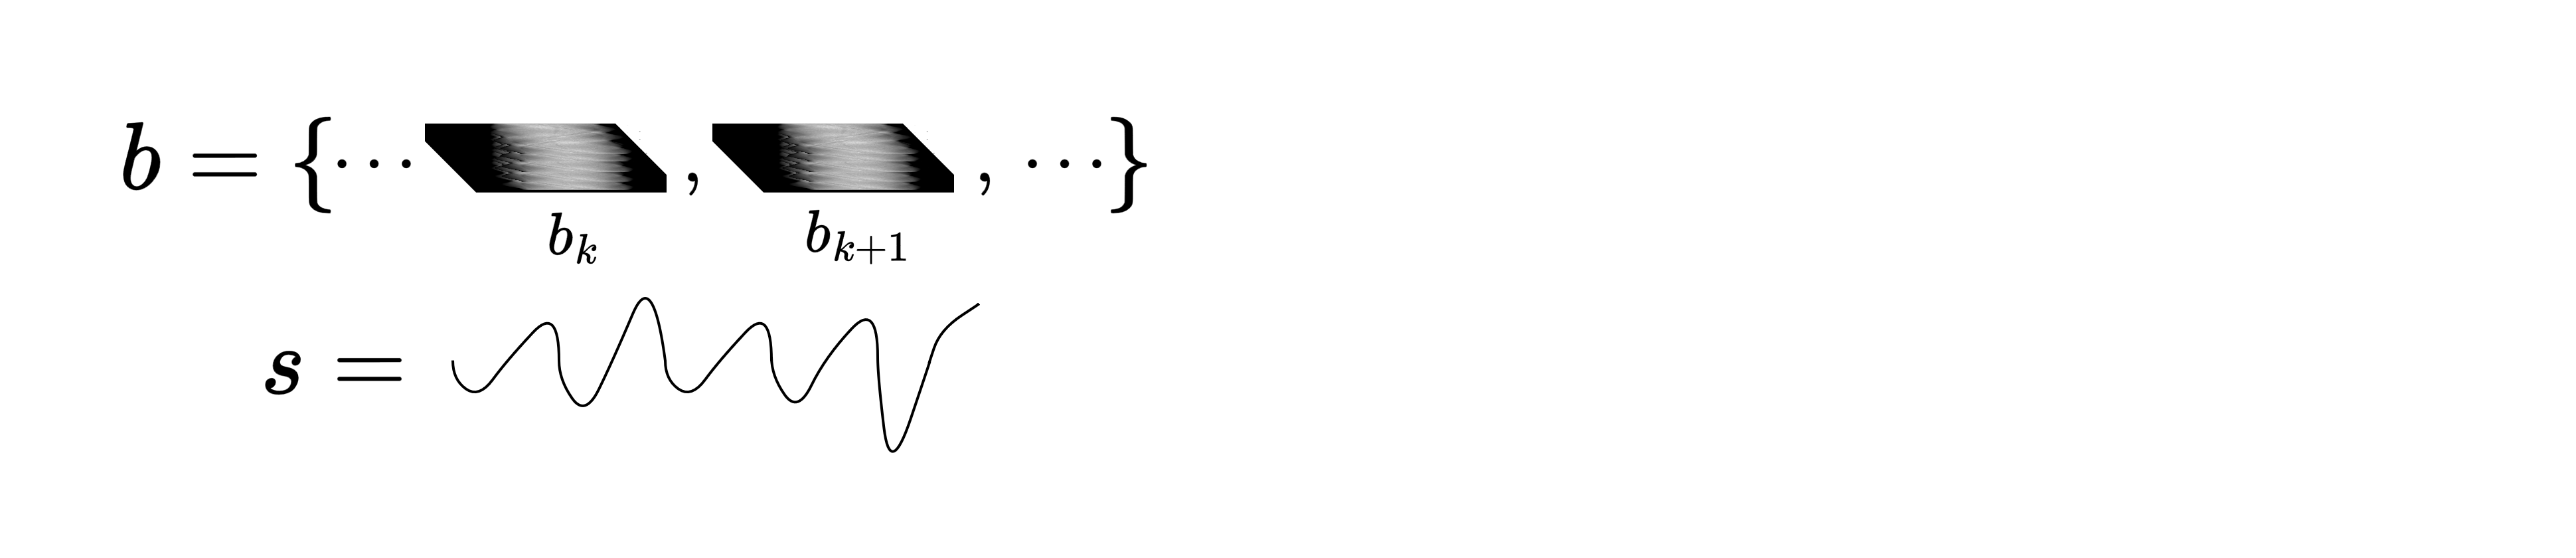
\includegraphics[width=1\linewidth]{figures/intro/gating_reco/gating1.png}}
  \only<2>{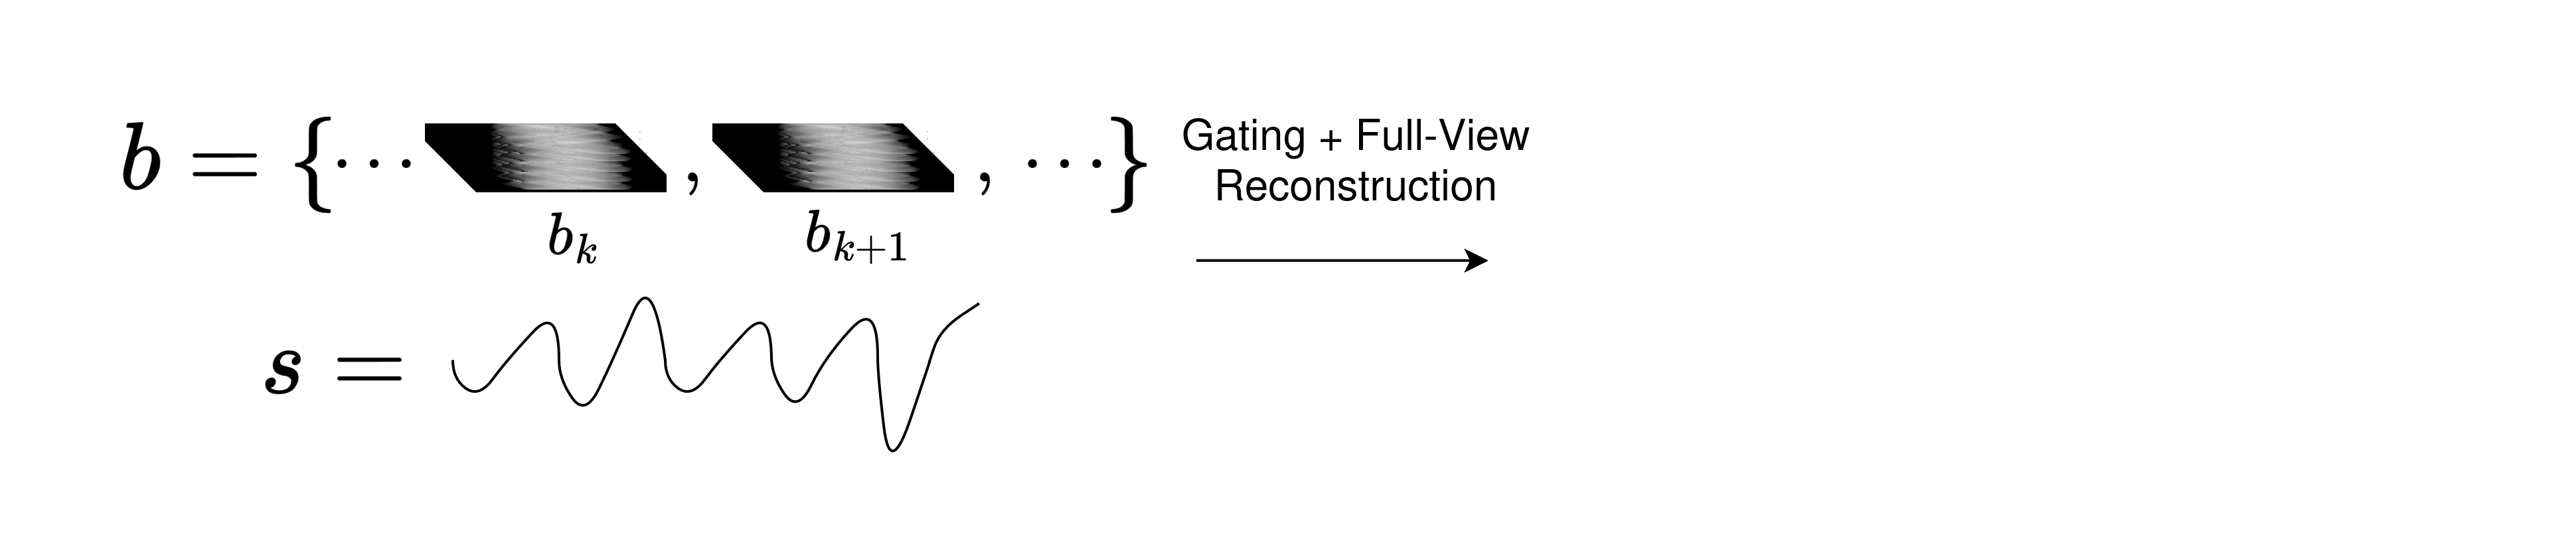
\includegraphics[width=1\linewidth]{figures/intro/gating_reco/gating2.png}}

  % Keep third image from slide 3 onwards
  \only<3->{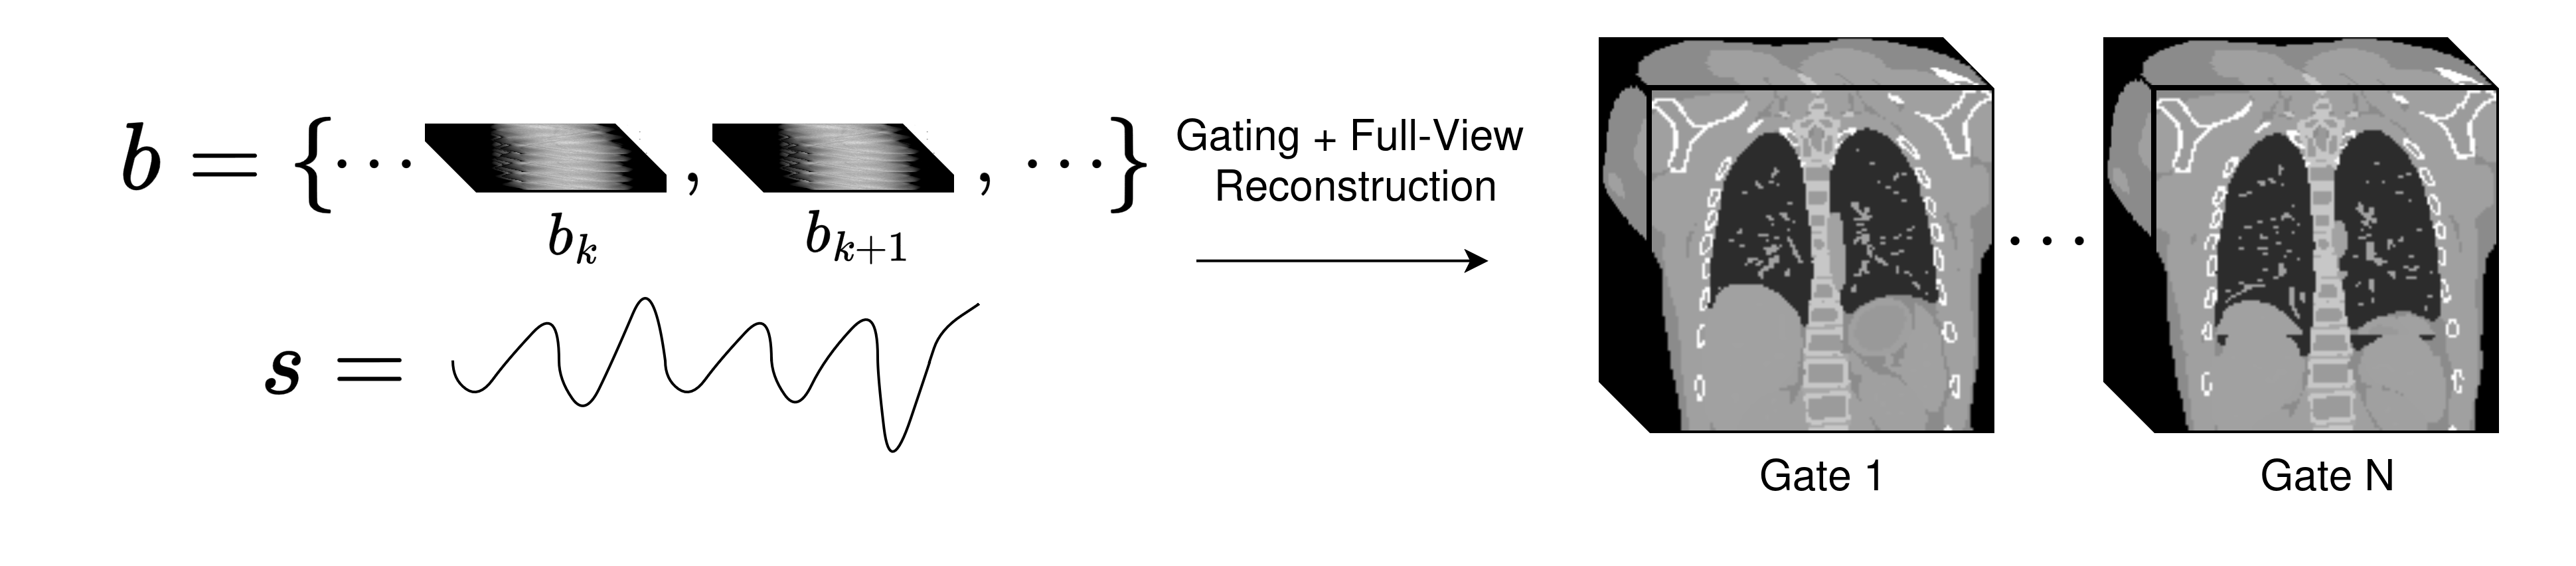
\includegraphics[width=1\linewidth]{figures/intro/gating_reco/gating3.png}}

  \vspace{0.3cm}

  \only<4->{
    \begin{itemize}
      \item<4-> \textbf{Challenges:}
            \begin{itemize}
              \item Motion artifacts due to irregular breathing patterns.
              \item Surrogate signals may not always be stored.
              \item Increased radiation dose from multiple phase acquisitions; necessitates dose reduction strategies.
            \end{itemize}
    \end{itemize}
  }
\end{frame}


\begin{frame}[t, fragile]
\frametitle{Joint Reconstruction \& Motion Estimation (JRM)}

    \begin{itemize}
    \item<1-> \textbf{General JRM Framework:}
              \begin{equation*}
              \min_{\textcolor{green}{\boldx},  \textcolor{orange}{\bold{\varphi}}} \frac{1}{2}\left\| \boldcalA_{\textcolor{orange}{\bold{\varphi}}} \textcolor{green}{\boldx} - \boldb \right\|_{W}^2 + \boldR(\textcolor{green}{\boldx})
            \end{equation*}

            where $\textcolor{orange}{\bold{\varphi}}$ are motion parameters.

      \item<2-> \textbf{4DCT JRM Framework \cite{huang2024resolving}:}
            \begin{equation*}
              \min_{\textcolor{green}{\boldx},  \textcolor{orange}{\boldphi}, \textcolor{orange}{\bolds}} \frac{1}{2}\sum_{k = 1}^{n_t}\left\| \boldcalR \circ \boldcalT_{k} \circ \boldcalW_{\textcolor{orange}{\boldphi} \cdot \textcolor{orange}{\bolds_k} } \textcolor{green}{\boldx} - \boldb_k \right\|_{W}^2 + \boldR(\textcolor{green}{\boldx})
            \end{equation*}

            \only<3>{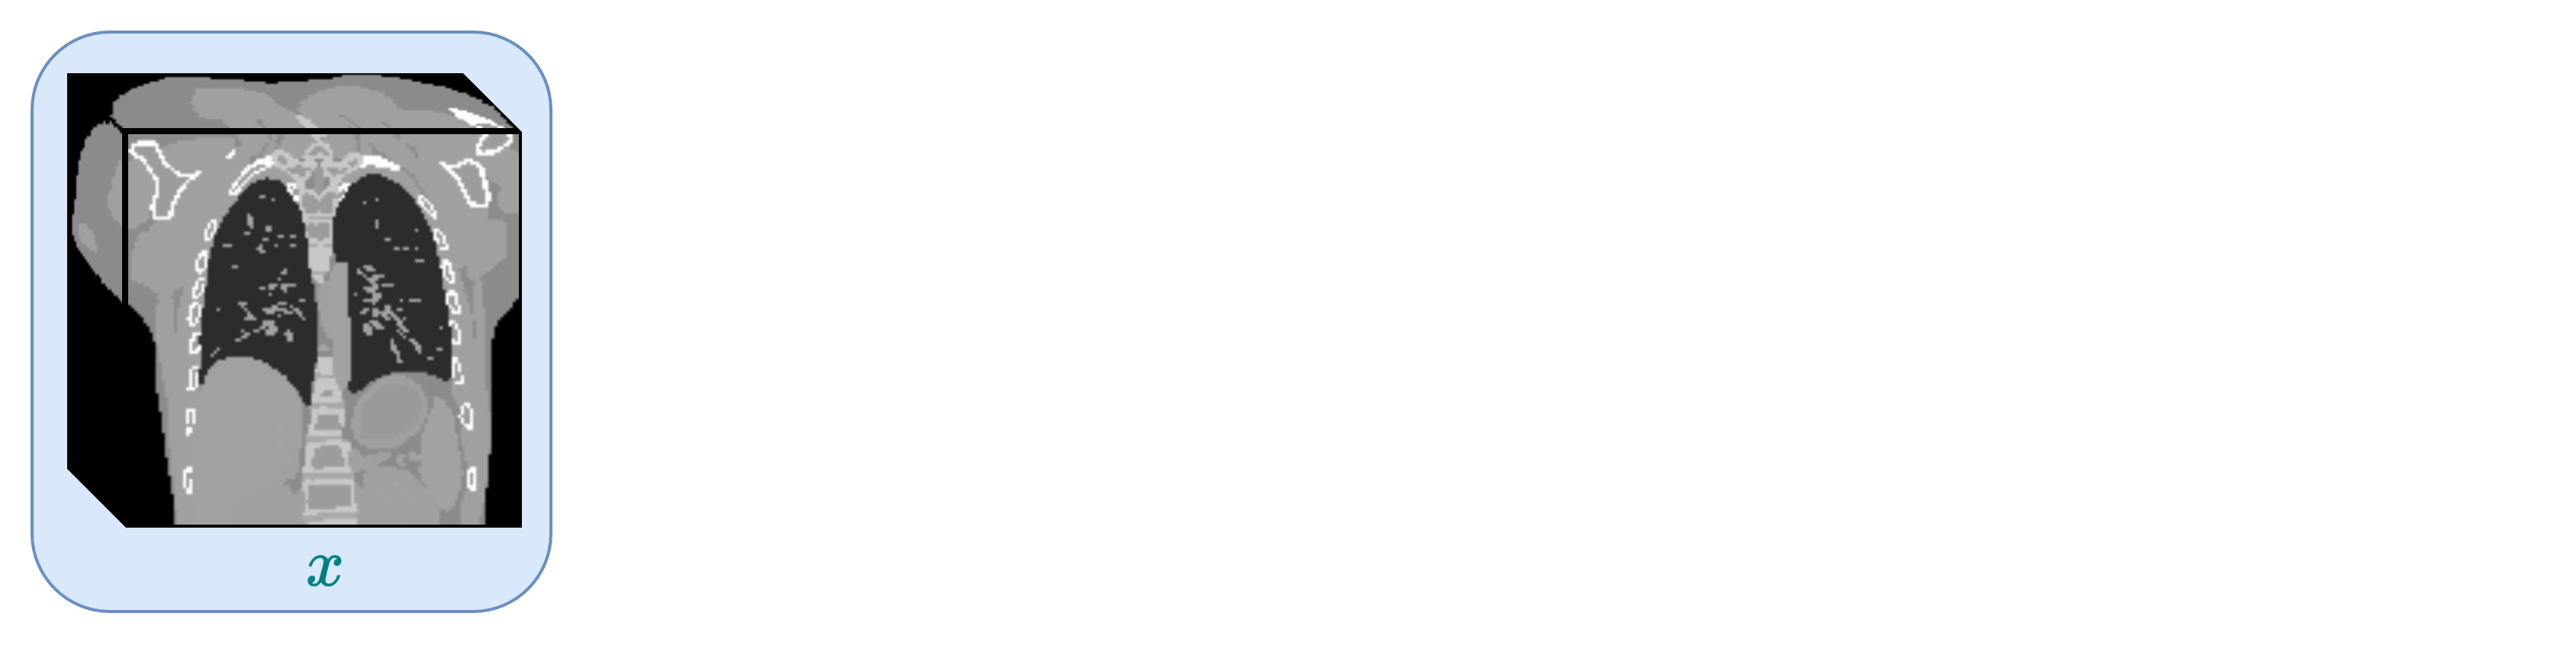
\includegraphics[width=1.0\linewidth]{figures/intro/blindforward/blindforward1.png}}
            \only<4>{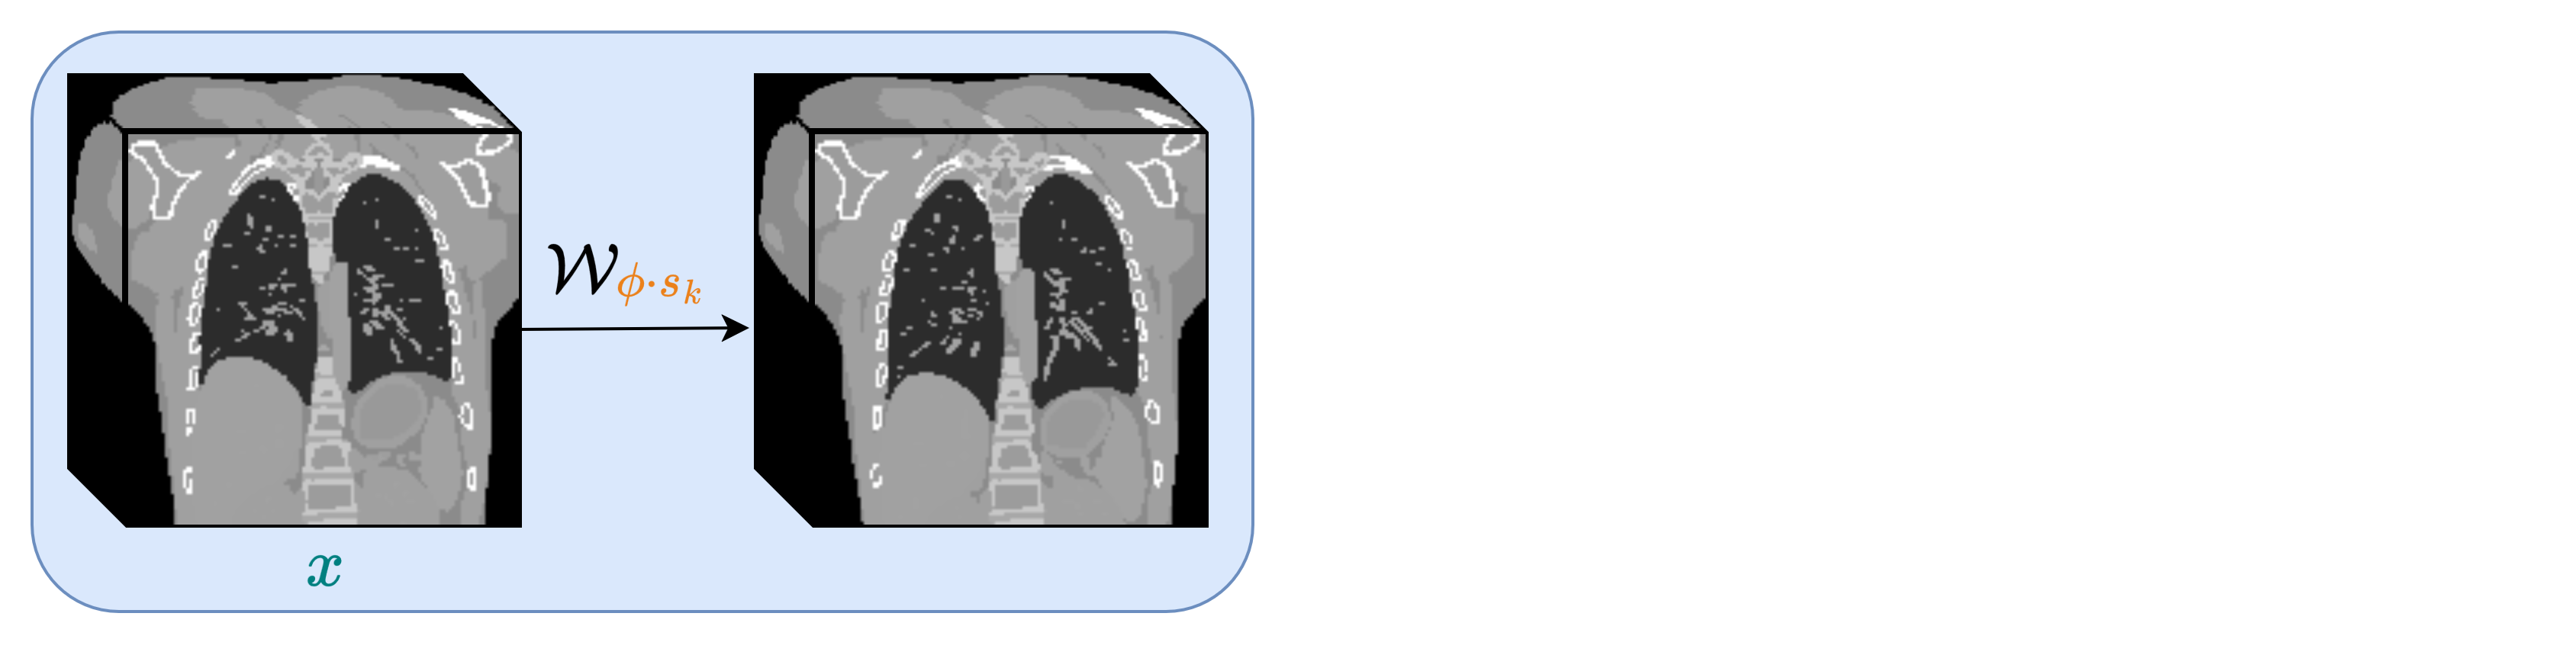
\includegraphics[width=1.0\linewidth]{figures/intro/blindforward/blindforward2.png}}
            \only<5>{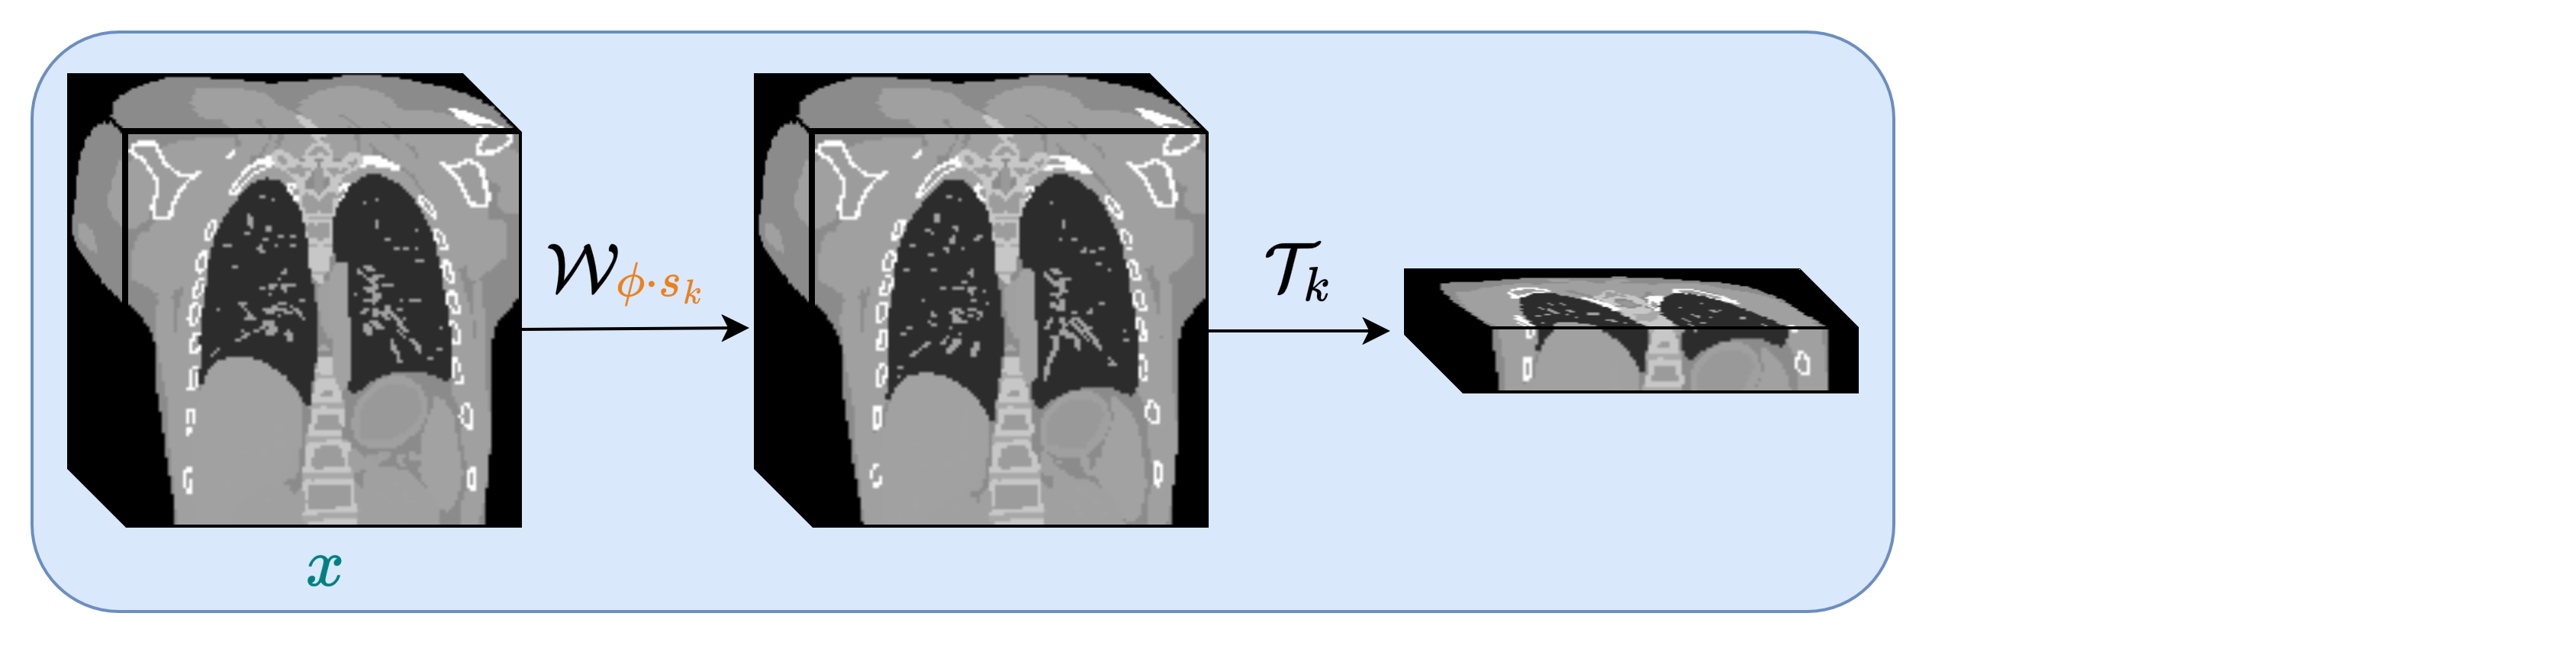
\includegraphics[width=1.0\linewidth]{figures/intro/blindforward/blindforward3.png}}
            \only<6>{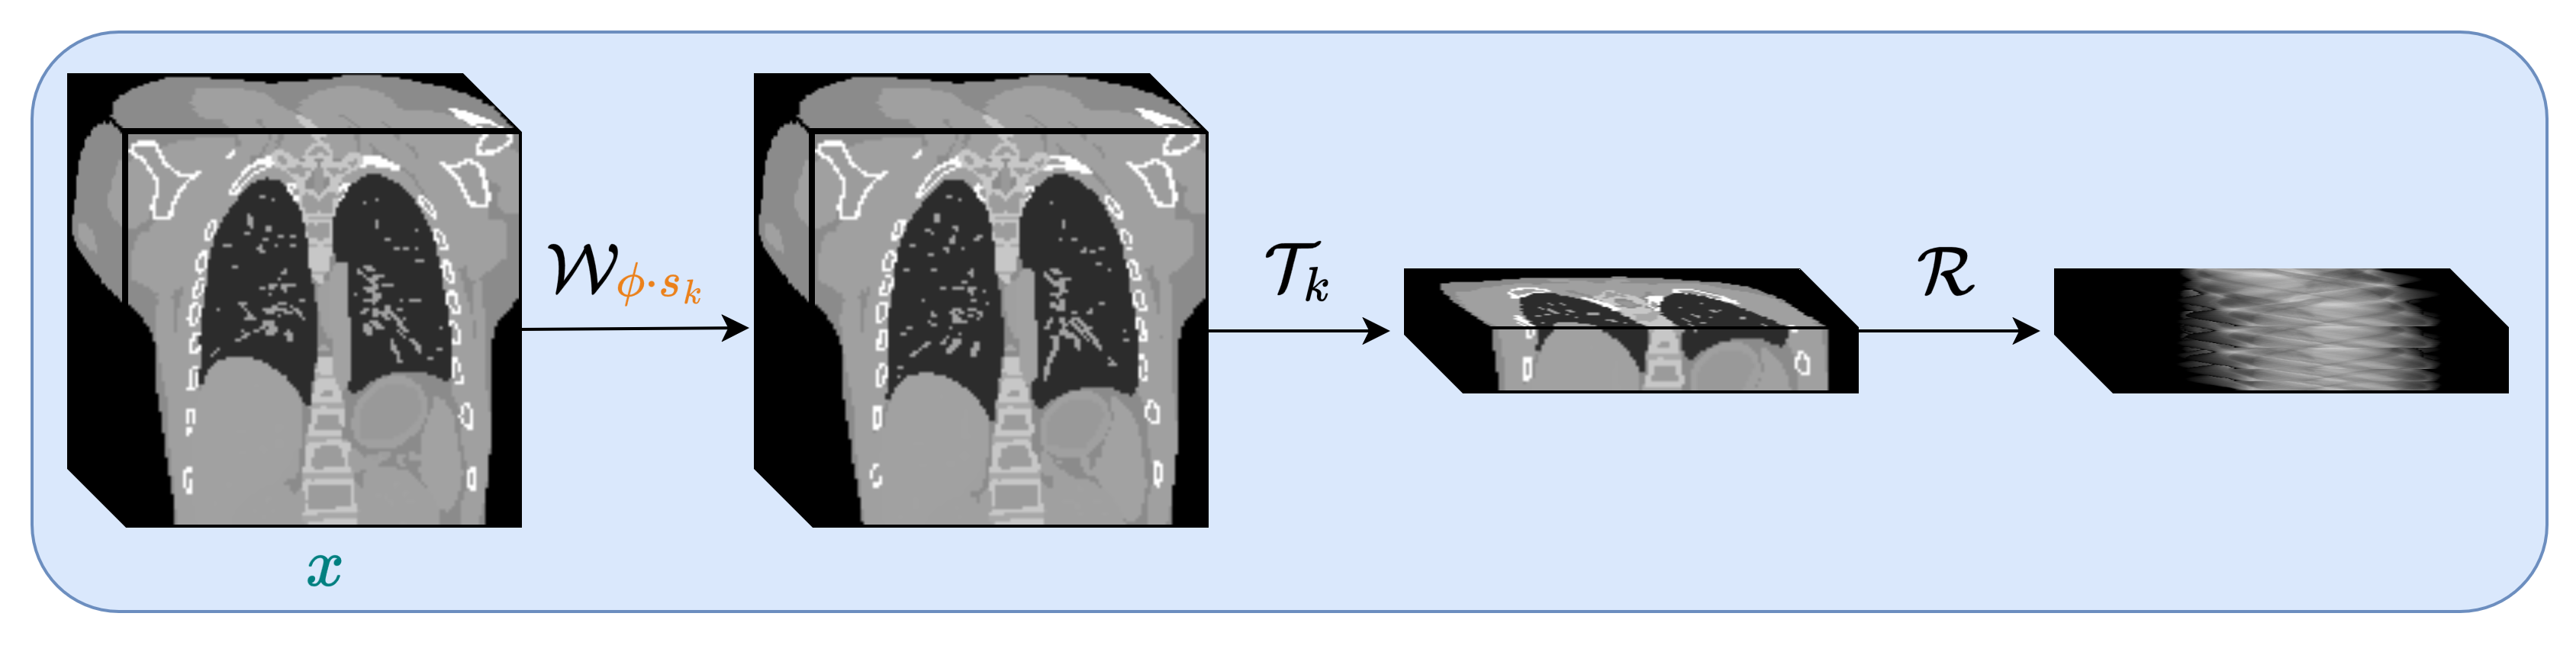
\includegraphics[width=1.0\linewidth]{figures/intro/blindforward/blindforward4.png}}
            where $\textcolor{orange}{\boldphi}, \textcolor{orange}{\bolds}$ are deformation vector fields parametrized by B-spline grid and surrogate signals.
            \vspace{0.5cm}
    \end{itemize}
\end{frame}
